The contributions of this paper is as follows:
\begin{itemize}
    \item A new ASR-free method is proposed, which can be applied in both "read aloud" and "open response" scenarios, and shows superior performance than previous methods that even using ASR. 
    \item Formulate the difference between ASR-free and w. ASR is the source of the speech segment boundary. From this perspective, we deeply analyze and understand why the SSL speech feature can work well in the fluency scoring task.  
    % The MFCC feature is introduced as a reference to illustrate the importance of highly representative feature.
\end{itemize}

\begin{table}[t!]
\centering
\small
\begin{tabular}{ccc|c}
\toprule
\multicolumn{3}{c|}{w. FA system}       & \multirow{2}{*}{Proposed} \\ \cline{1-3}
human  & $ASR_{online}$ & $ASR_{libri}$ &                           \\ \midrule
0.8117 & 0.7908         & 0.7607        & \textbf{0.7991}                    \\ \bottomrule
\end{tabular}
\caption{ASR-free vs. w.FA systems with different WERs.}
\label{tab:asr_error_effect}
\end{table}

\begin{table}[t!]
\centering
\caption{Performance of \textit{SSL\_idx} derived segment boundary and other counterparts on the MFCC input feature.}
\small
\begin{tabular}{cccc}
\toprule
\multicolumn{4}{c}{Segment Boundary Source}                                  \\ \hline
\multicolumn{3}{c|}{w/o ASR}                     & w. ASR           \\ \hline
\textit{N.A.}   & \textit{MFCC\_idx} & \multicolumn{1}{c|}{\textit{SSL\_idx}} & \textit{F.A.}\\ \hline
0.6672 & 0.7071   & \multicolumn{1}{c|}{0.7568}  & 0.7597           \\ \bottomrule
\end{tabular}

\label{tab:ssl_idx_on_mfcc}
\vspace{-3mm}
\end{table}

\begin{table}[ht!]
\centering
\caption{Top-5 cluster index assignment of several phones, the percentage in parentheses denotes the coverage ratio.}
\small
\begin{tabular}{c|c|c}
\toprule
Phone & train set             & test set              \\ \midrule
SIL       & 20,7,6,15,31 (59\%)   & 20,7,6,15,31 (57\%)   \\ \hline
IY        & 35.28,3,17,13 (71\%)  & 35,28,3,17,13 (71\%)  \\
IH        & 28,3,35,27,16 (70\%)  & 28,3,35,27,16 (70\%)  \\ \hline
B         & 10,23,26,11,15 (67\%) & 10,23,26,11,15 (66\%) \\
P         & 12,10,26,11,25 (68\%) & 12,10,26,11,25 (68\%) \\ \bottomrule
\end{tabular}

\label{tb:idx_stats}
\end{table}


\begin{table}[t!]
\centering
\caption{The summary of statistics of corpus ByteQA.}
\resizebox{\columnwidth}{!}{
\begin{tabular}{c|ccc}
\toprule
Data sets              & train           & dev           & test          \\ \midrule
\# of Spks             & 161             & 53            & 55            \\
\# of Utts             & 4404            & 1395          & 1451          \\ \midrule
\multirow{2}{*}{Total} & Avg \# of words & Avg dur (sec) & Max dur (sec) \\
                       & 33              & 22.2          & 172.5         \\ \bottomrule
\end{tabular}
}
\label{tab:dataset}
% \vspace{-4mm}
\end{table}


\begin{table}[t!]
\centering
\caption{Performance comparison between previous methods and the proposed one on the ByteQA dataset.}
\resizebox{\columnwidth}{!}{

\begin{tabular}{cc|cc|c}
\toprule
\multicolumn{2}{c|}{Methods}                                              & ASR-free & Text source & PCC   \\ \midrule
\multicolumn{1}{c|}{\multirow{3}{*}{\textrm{I}}} & FBDS-based fluency feature \cite{fontan2020using}   & \cmark & \xmark            & 0.549 \\
\multicolumn{1}{c|}{}                     & Prosodic + Disfluency feature \cite{deng2020automatic} & \xmark        & human       & 0.690 \\
\multicolumn{1}{c|}{}                     & Deep feature + w. FA  \cite{fu22b_interspeech}        & \xmark        & human       & 0.759 \\ \midrule
\multicolumn{1}{c|}{\multirow{2}{*}{\textrm{II}}} & SSL + w. FA                   & \xmark        & human       & 0.812 \\
\multicolumn{1}{c|}{}                     & SSL + w. FA                   & \xmark        & asr         & 0.791 \\ \midrule
\multicolumn{1}{c|}{\multirow{2}{*}{\textrm{III}}} & Proposed                      & \cmark        & \xmark           & \textbf{0.799} \\
\multicolumn{1}{c|}{}                     & Proposed \textbf{\textbackslash} cluster index   & \cmark        & \xmark           & 0.783 \\ \bottomrule
\end{tabular}

}
\label{tab:compare_with_baselines}
% \vspace{-2mm}
\end{table}


\begin{figure*}[ht!]
    % \vspace{-8mm}
	\centering
	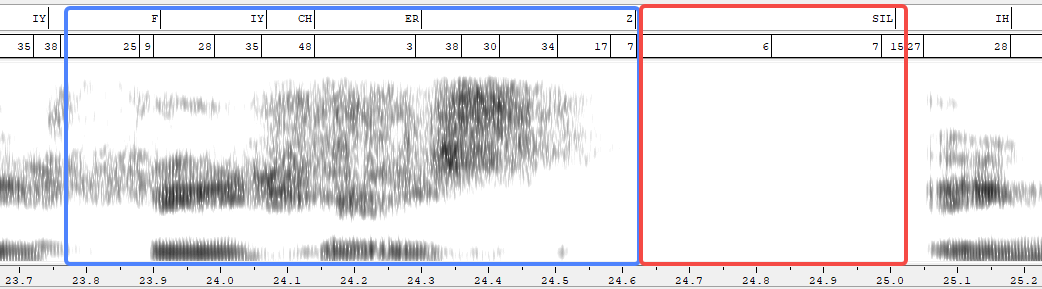
\includegraphics[width=150mm]{content/figs/ssl_idx_new.png}
	\caption{An example audio clip of corpus ByteQA with spoken content ``\textit{features}". Visualization of the phone boundary (top row bar) derived from forced alignment , and the segment boundary (second row bar) derived from the SSL cluster index.}
	\label{fig:ssl_idx}
\end{figure*}
